\chapter{UCNA Experiment}
\label{ch:UCNA_Experiment}
%%%%%%%%%%%%%%%%%%%%%%%%%%%%%%%%%%%%%%%%%%%%%%%%%%%%%%%%%%%%%%%%%%%%%%%%%%%%%%%
%%%%%%%%%%%%%%%%%%%%%%%%%%%%%%%%%%%%%%%%%%%%%%%%%%%%%%%%%%%%%%%%%%%%%%%%%%%%%%%
%%%%%%%%%%%%%%%%%%%%%%%%%%%%%%%%%%%%%%%%%%%%%%%%%%%%%%%%%%%%%%%%%%%%%%%%%%%%%%%

The UCNA Experiment is a mature experiment, having taken data from
2007-2013, that aims to precisely determine a value of $A_{0}$, the neutron
$\beta$-decay asymmetry parameter. Here a description of the experimental
apparatus is given, as well as previous measurements
of $A_{0}$ from other experiments for comparison.

The description which follows applies to data taken from Fall 2011 through
Spring 2013. The analysis is split into two separate data sets, 2011-2012
and 2012-2013, due to minor changes in the decay trap geometries. Although
small, any changes in the geometry prompt new simulations, and so a separate
analysis is carried out. From now on, any part of the experiment or analysis
which is different for the two data sets will be indicated.

\section{Overview}
\label{sec:Overview}

The goal of UCNA is to produce UCN in a solid deuterium source which is fed
neutrons via a spallation source at the end of an $800$ MeV
proton beam. These UCN are then guided towards a material trap where they can
decay. During travel, the UCN pass through a series of polarizing magnets
which allows the experimenter to control the spin state of the neutrons in
the trap during any run. Utilizing a strong $~1$~T magnetic field in the
decay volume, decay electrons are guided towards detectors at either end of
the decay volume where their energy can be reconstructed. From knowledge about
the initial direction and the energy of the neutron, one can construct an
energy dependent asymmetry and determine a value for $A_{0}$.

%%%%%%%%%%%%%%%%%%%%%%%%%%%%%%%%%%%%%%%%%%%%%%%%%%%%%%%%%%%%%%%%%%%%%%%%%%%%%%%
%%%%%%%%%%%%%%%%%%%%%%%%%%%%%%%%%%%%%%%%%%%%%%%%%%%%%%%%%%%%%%%%%%%%%%%%%%%%%%%
\section{Ultracold Neutron Source and Guide System}
Detailed descriptions of the UCN source can be found in
\cite{saunders2004demonstration,morris2002measurements,saunders2013performance}, with
more recent improvements given in \cite{ito2017performance}.

The creation of UCN begins with delivery of protons from the 800~MeV proton
accelerator operated in pulsed mode, with pulses repeated at a rate of 0.2~Hz.
The protons strike a helium-cooled tungsten target (12~cm long) and produce
spallation neutrons at roughly 20~MeV. The spallation target is surrounded by
a room temperature beryllium reflector to help direct as many neutrons as
possible towards the UCN source. The solid deuterium ($\mathrm{SD}_2$) UCN source
is located directly above the tungsten target and is housed in a liquid helium
cooled cryostat. Prior to entering the $\mathrm{SD}_2$ source, neutrons
pass through a 1~cm thick moderator made of polyethylene beads cooled with the boil off gas
from the cooling of the $\mathrm{SD}_2$ source in the cryostat.

The $\mathrm{SD}_2$ source is a cylinder 19.7~cm in diameter and 5.7~cm tall. There
are a collection of ``fins'', or vertical teeth-like structures, located in
the bottom of the aluminum cryostat to increase the surface area of contact between the
$\mathrm{SD}_2$ and the liquid helium cooled surface. The surface of the cryostat
is coated with beryllium to reflect as many UCN as possible within the UCN source. Above
the $\mathrm{SD}_2$ is a flapper valve which opens to let UCN out of the source and
prevents UCN from re-entering the $\mathrm{SD}_2$ to reduce upscattering and loss of UCN.

Once a UCN passes the flapper, it is guided along a 1~m vertical guide coated with $^{58}\mathrm{Ni}$.
At this point, the UCN enter stainless steel horizontal guides to be transported from
the biological shielding that surrounds the source. The higher 342~neV potential of the
the $^{58}\mathrm{Ni}$ ensures that all neutrons which are capable of being guided by the
stainless steel (189 neV potential) are trapped at bottom of the vertical guide
\cite{saunders2013performance}. Upon looking at figure \ref{fig:guides}, one sees that
there are two $45\degree$ bends in the stainless steal guides to remove neutrons still
exceeding the UCN regime \cite{plaster2012}.

\begin{figure}[h]
  \centering
  \includegraphics[scale=0.48]{2-UCNAExperiment/experimentalSetup.png} 
  \caption{Schematic of guides and layout of the UCNA experiment \cite{plaster2012}.}
  \label{fig:guides}
\end{figure}

Once the UCN exit the shielding, they are guided along stainless steel guides
through a gate valve which allows for separation of the UCNA apparatus from the UCN
source while the proton beam is on, thus allowing for background measurements in
the spectrometer
during $\beta$-decay running conditions (proton beam operating, but void of UCN).
Beyond the gate valve is a 6~T pre-polarizing magnet (PPM). The purpose of the PPM
was to minimize the loss of UCN during transport through the Zr foil used to separate
the vacuum in the UCN source from the vacuum in the rest of the apparatus. The neutrons
are nominally polarized longitudinally after passing through the PPM's longitudinal field.

Beyond the PPM, the guides switch to electropolished copper (168 neV potential) to
maintain the initial polarization of the neutrons. Just downstream of the PPM
is the ``switcher'' valve. When the valve is open, the downstream guides are connected
to the guides coming from the PPM carrying UCN. Upon closing the switcher valve,
the downstream guides are redirected to a $^3\mathrm{He}$ 
UCN detector \cite{morris2009multi} used in polarimetry measurements.

Beyond the switcher,
the UCN are guided through the 7~T primary polarizing magnet (or AFP magnet). At this point
the guides switch to 100~cm of diamondlike carbon coated quartz guides \cite{mammei2010thin}
for passage through the Adiabatic Fast Passage (AFP) spin flipper \cite{holley2012high}. Again
the guides switch back to circular copper guides before coupling to a rectangular
(4~cm width $x$ 7~cm height) copper guide which transports the neutrons into the 1~T field
inside the Superconducting Spectrometer (SCS).

Prior to the beginning of running in 2011, a shutter was installed between the decay trap and
the guides used to close the decay trap off from the guides. During normal $\beta$-decay
runs, the shutter is open allowing neutrons to flow into (and out of) the decay trap as they are
created in the source. The shutter is closed at the beginning of a depolarization run, which immediately
follows every $\beta$-decay run, to allow for draining of the guides prior to a depolarization
measurement. This will be discussed in more detail later.

\section{Polarization}

The neutrons are initially polarized utilizing the $\boldsymbol{-\mu\cdot B \approx \pm 60}$~neV/T
potential. The UCN pass through the 6~T pre-polarizing magnet and then
pass through the 7~T primary AFP polarizing magnet. Neutrons with spin
aligned to the field (remember that the magnetic moment of the neutron is negative and so is antialigned
to the spin) see a positive (repulsive) potential of 420~neV from the 7~T megnet, and thus all
UCN in this spin state will be reflected. The opposite spin state will be transmitted, thus producing
a completely polarized population of UCN beyond the AFP magnet.

At this point, the neutrons pass through the AFP spin flipper. If the spin flipper is on, the spins
undergo a $\pi$ spin flip before being loaded into the decay trap, and if it is off, the spins are
loaded in the same state that was selected by the AFP magnet.

A detailed description of the spin flipper can be found in \cite{holley2012high}. In short, the
flipper works under the premise of nuclear magnetic resonance (NMR) and utilizes a sinusoidally
varying magnetic field ($B_1$) that is transverse to the primary holding field ($B_0\approx 1$~T).
A gradient is introduced in the holding field $B_0$ such that the rotating field $B_1$ is on resonance
with the larmor precession of the neutron's spin about the holding field. As such, upon traversal over
the entire flipper geometry, meeting this resonance condition guarantees a spin flip for the majority of
UCN. Testing of the apparatus indicates an efficiency of $0.9985\pm0.0004$ \cite{holley2012high}.

\begin{figure}[h]
  \centering
  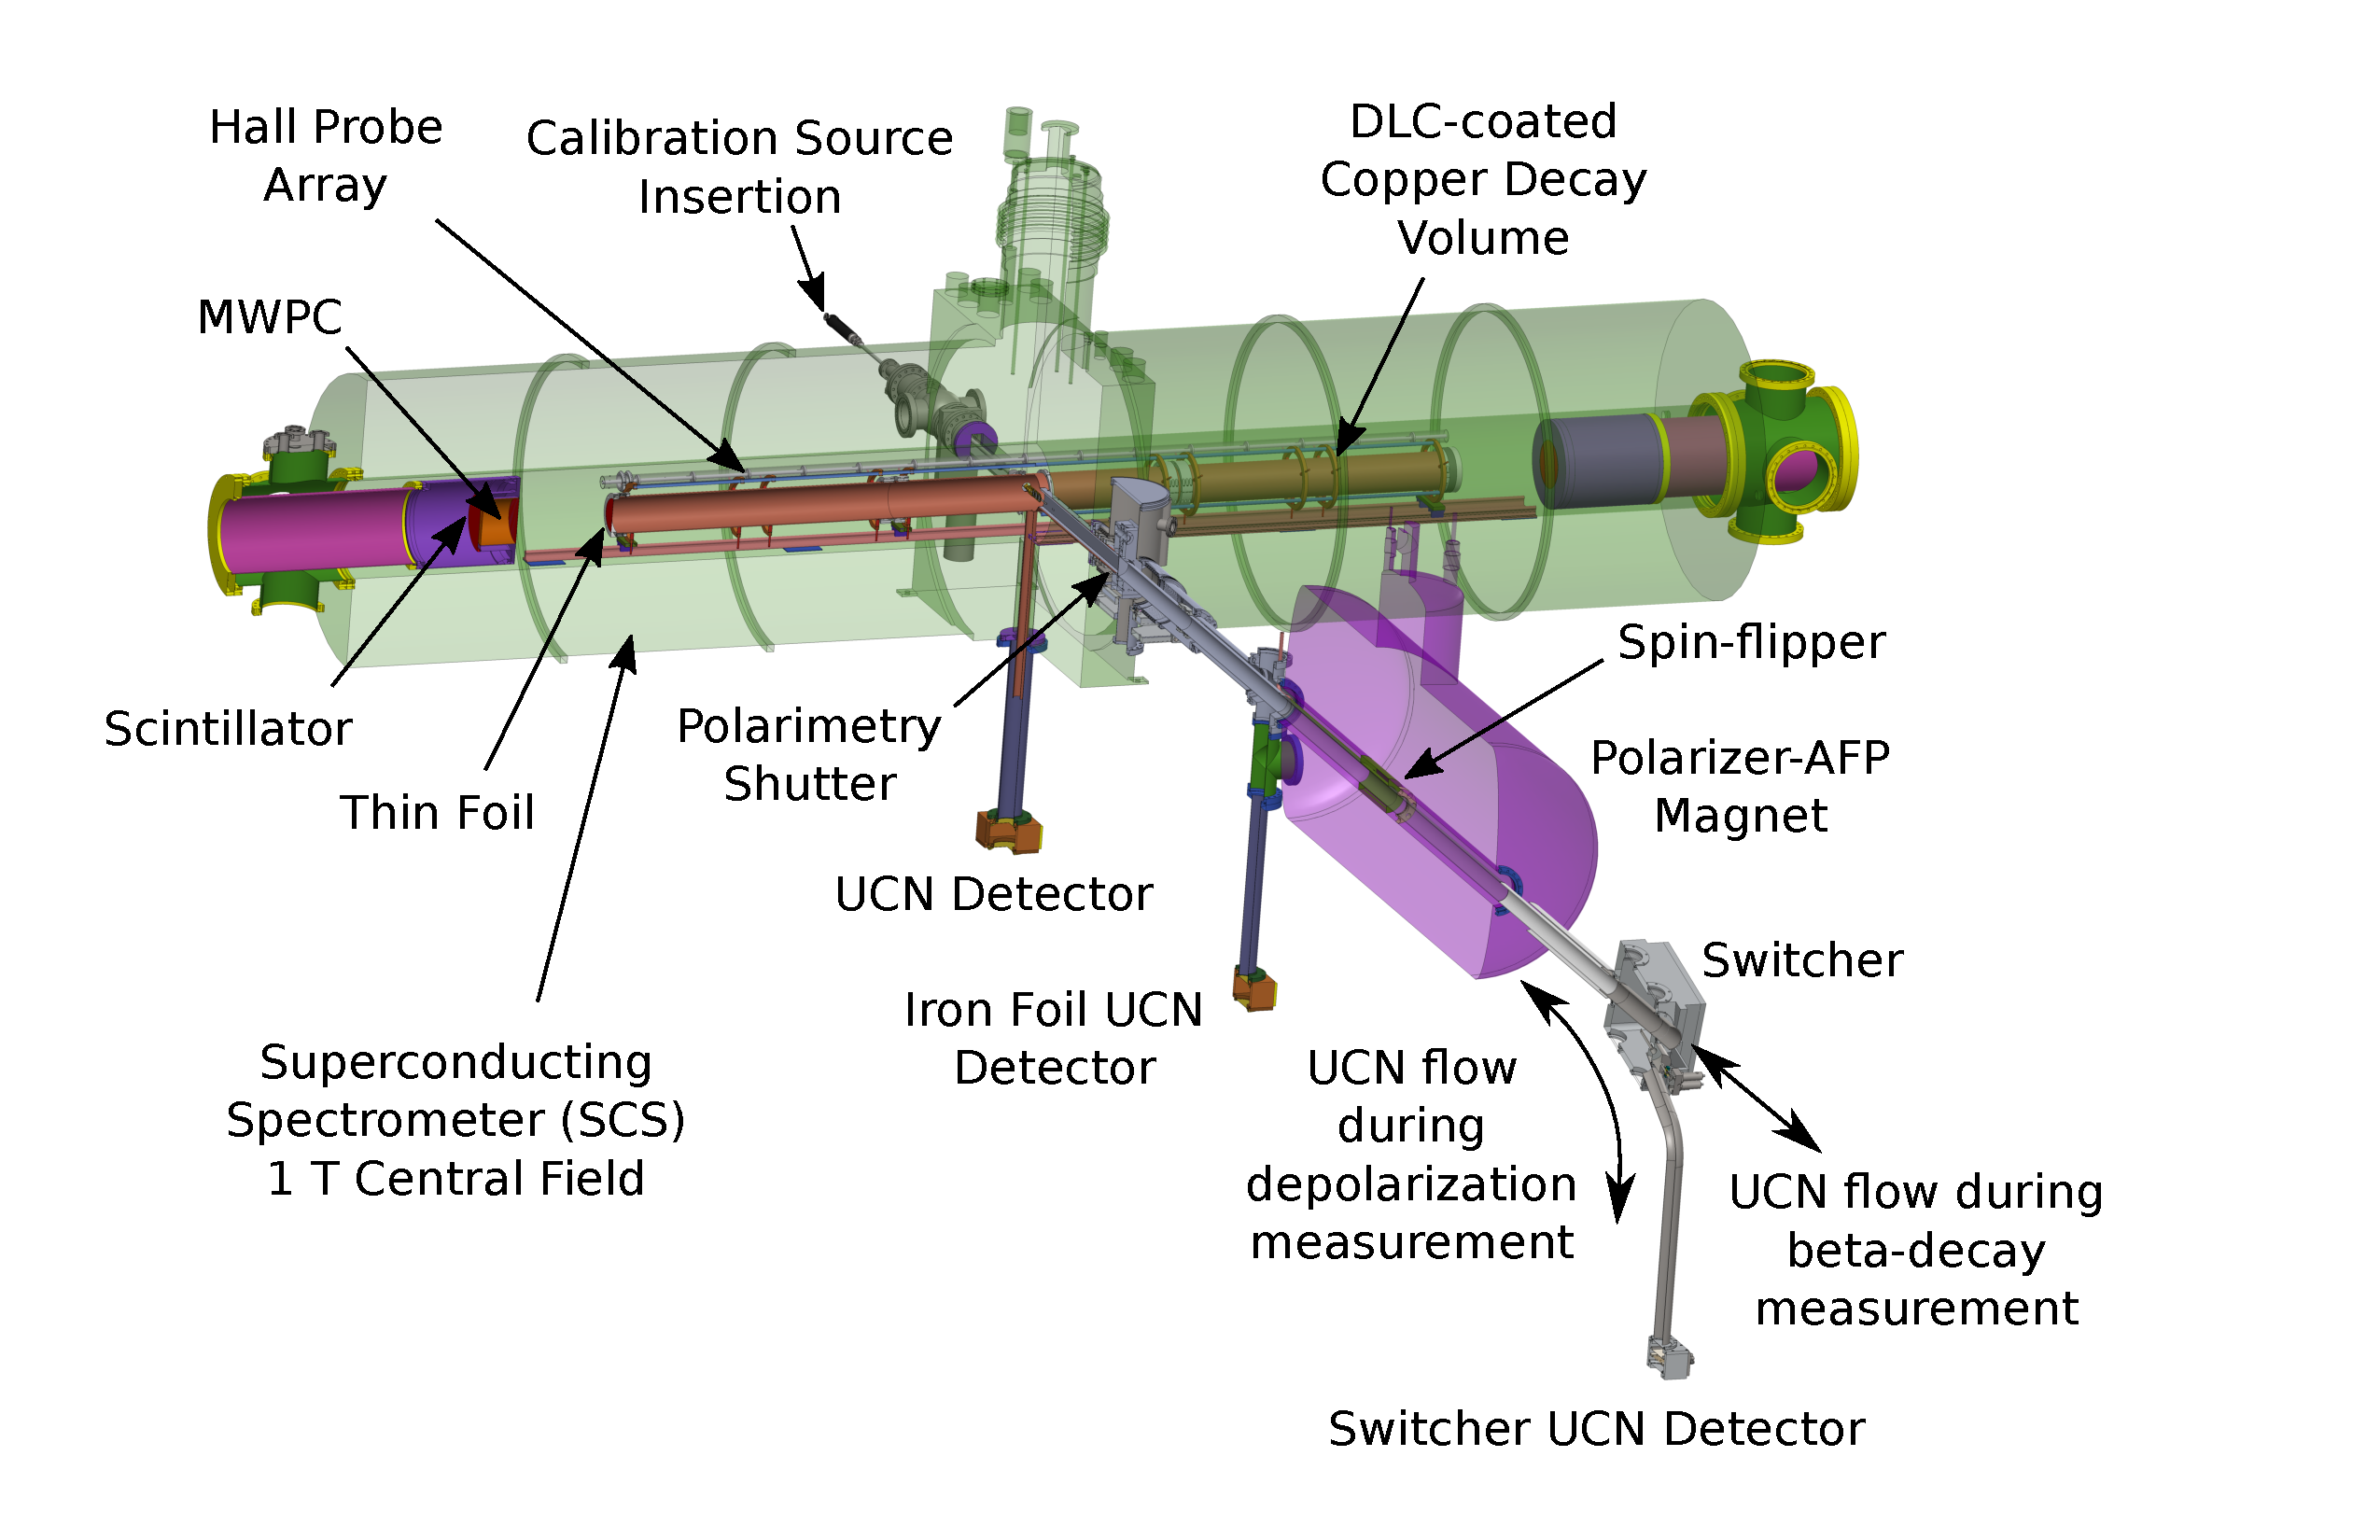
\includegraphics[scale=0.38]{2-UCNAExperiment/UCNAFig.pdf} 
  \caption{Detailed rendering of the experimental area. }
  \label{fig:setup}
\end{figure}

\section{Super-conducting Solenoidal Spectrometer}

The spectrometer consists mainly of the superconducting solenoidal magnet designed to produce
the 1~T central field, a decay trap to contain the UCN until they decay, and detector
packages located at each end of the spectrometer to detect decay electrons after they spiral
about the field lines towards either detector. The detectors are often described as
East and West based on their orientaion in the experimental area. Brief descriptions of the main components follow.

\subsection{Decay Trap}
The decay trap is situated at the center of the spectrometer within the 1~T magnetic
field. The cylindrical 300 cm in length, 12.4 cm in width decay trap is made of electropolisged Cu
to confine as many UCN as possible. Typically the vacuum within the decay trap and the guides
upstream until the Zr foil which separates the source vacuum from the experimental apparatus is about
$10^{-5}$~Torr. The density of UCN in the decay trap was monitored using a $^3He$ UCN detector
directly below a 0.64~cm hole in the decay trap.

One of the main differences between the 2011-2012 and 2012-2013 run periods is the thickness and
material of the decay trap endcaps. In both geometries the endcaps are coated with 150~nm of
Be (potential 252 neV) to aid in reflecting neutrons to confine them. The 2011-2012 endcaps
were 500~nm Mylar on both the East and West detectors, while the 2012-2013 endcaps were made of 6F6F
\cite{hoedl2003} and were 130~nm (East) and 180~nm (West) thick. The change in endcap thickness
is the primary reason for analyzing the two sets of data separately, as this changes the
systematics involving electron backscattering. 

\subsection{Magnetic Field} \label{ssec:MagneticField}

The general idea for the magnetic field within the decay trap is that it must be aligned with
the axis of the decay trap to define the axis of polarization, strong enough to confine the larmor
radius of the decay electrons as they spiral toward the detectors, and uniform enough that
electrons will not be reflected.

The necessity for a uniform magnetic field follows from consideration of the flux contained
within the spiral of the electron around the magnetic field lines. From \cite{jackson1999}
we know the flux, $Br_e^2$, is an adiabatic invariant, which means so is $p_\perp^2/B$ where
$p_\perp$ is the transverse momentum of the spiraling electron and $p = \sqrt{p_\perp^2+p_\parallel^2}$.
Given this, there exists a condition for reflection when an electron originates in a field $B_0$
with initial momentum $p_0 = \sqrt{p_{0,\perp}^2+p_{0,\parallel}^2}$
and encounters a field $B_{\mathrm{max}}$,
%
\begin{equation}
  \frac{B_{\mathrm{max}}-B_0}{B_0} > \frac{p^2_{0,\parallel}}{p^2_{0,\perp}}.
  \label{eq:fieldReflection}
\end{equation}
%
A field uniformity of $10^{-4}$ was determined sufficient to remove appreciable effect
on the asymmetry \cite{plaster2008solenoidal}.

The magnet, constructed by American Magnetics, Inc., is a warm-bore 35~cm diameter, 4.5~m
long superconducting solenoid (SCS magnet). Technical details of the magnet can be found in
\cite{plaster2008solenoidal, plaster2012}. An important aspect of the magnetic field not mentioned
previously is the field expansion from 1~T to 0.6~T beyond the decay trap windows but prior to
the wirechambers. This field expansion decreases the pitch angle of the electron as it
enters the detector package, defined as
$\theta = \arccos(p_{\parallel}/p)$, as seen from the earlier stated adiabatic invariant $p_\perp^2/B$
coupled with conservation of momentum. Decreasing the pitch angle decreases the probability
of backscattering substantially.

\begin{figure}[h]
  \centering
  
\includegraphics[scale=0.38]{2-UCNAExperiment/ImageHolder.pdf} 
  \caption{Typical field profile from 2011-2012 run period.}
  \label{fig:field_profile}
\end{figure}

In 2011-2012 and 2012-2013, the magnetic field was not as uniform as reported in 
\cite{plaster2008solenoidal} due to damage to the shim coil persistence heater switches
due to multiple magnet quenches \cite{plaster2012}. A typical field profile can be seen
in figure \ref{fig:field_profile}, where the uniformity is at the $10^{-3}$ level, but there is
pronounced dip in the center. Electrons
that originate in the dip region can become trapped if the condition in equation
\ref{eq:fieldReflection} is satisfied. The electron then only exits the field dip
upon scattering from the residual gas in the decay trap which randomized the direction
of the electron. The effect
on the asymmetry from the field
dip is addressed as a systematic
uncertainty in section \ref{sssec:MagFieldSyst}.


\subsection{Detector Packages}

\begin{figure}[h]
  \centering
  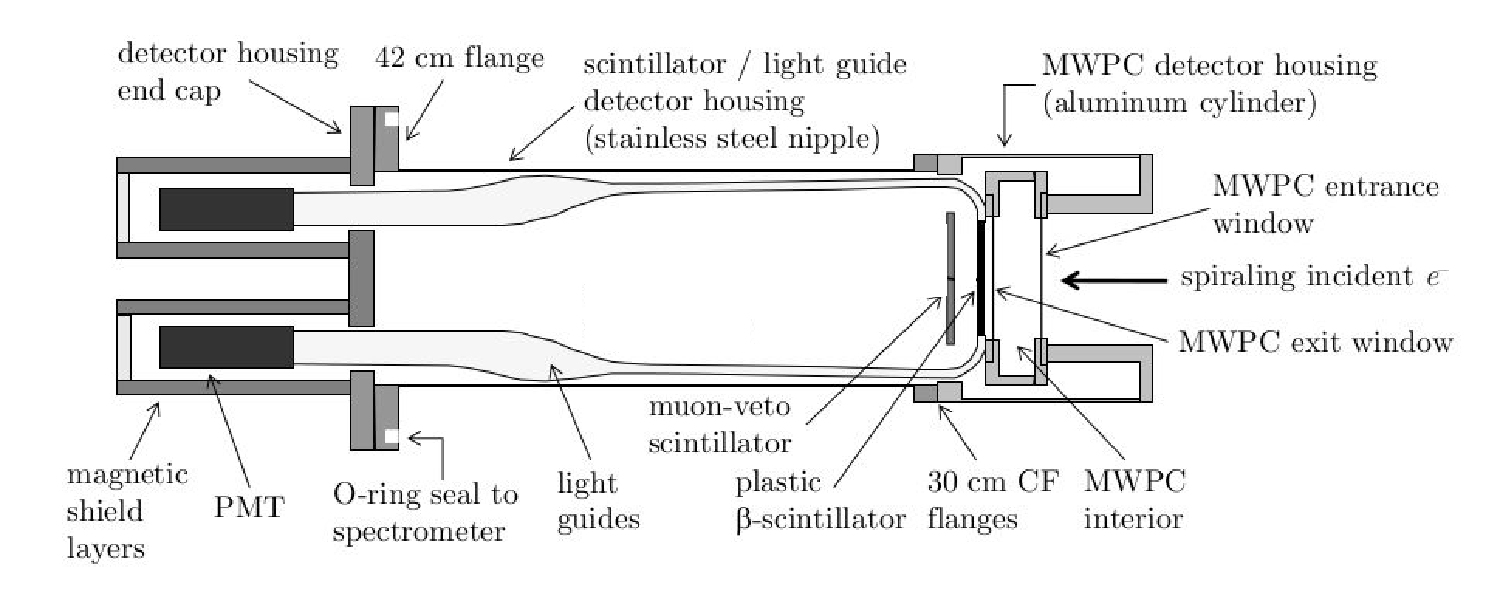
\includegraphics[scale=0.6]{2-UCNAExperiment/detector_setup.pdf} 
  \caption{Schematic of the detector packages \cite{plaster2012}.}
  \label{fig:detectors}
\end{figure}

\subsubsection{Multiwire Proportional Chamber}

The multiwire proportional chamber (MWPC, or sometimes simply called the wirechamber)
\cite{ito2007,plaster2012} is
utilized to reconstruct the position of the electron events and to reduce the ambient
backgrounds. The MWPC consists of an anode plane in between two cathode planes, with the cathode
planes oriented perpendicular to one another to allow for position reconstruction in both directions
transverse to the axis of the SCS. There are
64 wires in each plane with 2.54~mm spacing between each wire. The spatial extent of the
MWPC is $16.3 \times 16.3\mathrm{ cm}^2$ which maps to
$\sqrt(0.6) (\times 16.3 \times 16.3\mathrm{ cm}^2) = 12.6 \times 12.6\mathrm{ cm}^2$ coverage
within the decay trap (remember the decay trap is within the 1~T field while the detectors
are in the field expansion region with field of 0.6~T), thus the wirechamber covers the full
decay trap exit. The anode wires are $10\mathrm{ \mu{n}}$ in diameter while the cathode
wires are $78.2\mathrm{ \mu{n}}$ in diameter, with the diameter of the cathode wires slightly
larger than in previous run periods ($50\mathrm{ \mu{n}}$).

Charged particles passing the MWPC ionize the gas, and the \~2700~V bias between the anode and
cathode plains causes the ions and electrons to driftThe anode wires are read out as a summed signal, with all 64 wire signals summed corresponding to
a single ADC channel. This signal is typically used in relating the total signal in the MWPC
to an energy deposited within the wirechamber. The cathode wires are read out in groups of four
consecutive wires, so there are 16 ADC channels for each wirechamber cathode plane. These 16
``wires'' (as we will call them from now on) are used for position reconstruction. Either
signal can be effectively used for the MWPC software trigger.

The fill
gas chosen for the MWPC should be low Z ( low atomic number) to minimize the backscattering from heavy nuclei,
but also electron dense to increase the ionization efficiency. Thus complex large molecules
made up of low Z nuclei are good candidates.
The MWPC was primarily filled with neopentane ($\mathrm{C}_5\mathrm{H}_{12}$) gas at a pressure of
100~Torr, chosen to ensure enough gain for electrons within the $\beta$-decay spectrum. For a
short time period in 2012-2013, the neopentane ran out and isobutane ($\mathrm{C}_5\mathrm{H}_{10}$)
was used instead. Separate simulations were used for the isobutane runs, but no appreciable
difference was noticed.

The windows on the wirechamber were made as thin as possible so as to reduce backscattering, but still
retain their integrity under the 100~T pressure difference between the SCS and the wirechamber. Events that
scatter off of the entrance window are particularly troublesome as they become missed backscattering events.
The chosen front window material was $6\mathrm{ \mu{n}}$ of aluminized Mylar reinforced with Kevlar strings
placed at 5~mm increments, and the exit window was also $6\mathrm{ \mu{n}}$ of aluminized Mylar \cite{mpmThesis}. 

The importance of the MWPC should not be understated. First of all, the position reconstruction allows for the
definition of a fiducial volume within the decay trap so that we can cut out events which may have interacted
with the decay trap walls. Such interactions change the energy/direction of the electron, so simply cutting them
out reduces the systematic correction necessary. Secondly, the scintillator's energy response is position
dependent, so the position of each event is needed to properly assign a reconstructed initial energy to
each electron event. The MWPC is also vital in identifying backscattering events by looking at the energy
deposited within the wirechamber, i.e. an event that backscatters off of the dead layer of the scintillator
will deposit energy in the MWPC above some software cut and can be identified. And last of all,
the wirechamber is highly insensitive to gamma rays, so by including a coincidence trigger between the wirechamber
and the scintillator the majority of the gamma background is removed.

\subsubsection{Scintillator}

A 15~cm diameter, 3.5~mm thick plastic scintillator \cite{plaster2012}
from Eljen Technology (EJ-204) was located beyond the
MWPC. The maximum stopping distance for an endpoint (782~keV) electron is 3.1~mm, so the
scintillator is capable of reconstructing the entire energy spectrum. To transport the
scintillation light out of the 0.6~T field to the photomultuplier tubes (PMT),
located \~1~m in a \~0.03~T field,
twelve light guides were coupled to the edge of the scintillator using optical grease.
From there, the twelve guides are adiabatically merged into four
larger guides which are attached to four Hamamatsu R7725 PMTs with custom bases \cite{hickerson2013}.
The light guides are merged and coupled to the PMTs in such a way that each PMT effectively
covers one quadrant of the scintillator, as will become clear when discussing the calibrations.
A hardware two-fold trigger, or two PMTs above discriminator threshold, is required for an
global trigger to be issued from the PMTs.

\subsubsection{Energy Calibration}

The scintillator energy calibration utilized the conversion electron lines from
(with dominant K-shell energies listed) $^{137}\mathrm{Ce}$
(130.3 keV), $^{113}\mathrm{Sn}$ (363.8 keV), and $^{207}\mathrm{Bi}$ (481.7~keV and 975.7 keV)
sources. These sources were placed on a source paddle and inserted into the side of the
decay trap while under vacuum, and then they were translated across the horizontal axis of the decay
trap. This method probed the position dependence of the scintillator, but only along one axis and
at discrete points. The full position response was captured using another method as will be
described later. Also detailed later in section \ref{sec:biGain}, the gain of the PMTs was monitored
and drifts corrected 
on a run-by-run basis using a $^{207}\mathrm{Bi}$ ``pulser'' system \cite{morris1976stable}.

\subsubsection{Muon Veto System}

Cosmic ray muons can create a scintillator two-fold triggers and also pass the software trigger in
the MWPC, as they are charged particles.

\section{Data Acquisition}



%%%%%%%%%%%%%%%%%%%%%%%%%%%%%%%%%%%%%%%%%%%%%%%%%%%%%%%%%%%%%%%%%%%%%%%%%%%%%%







